\chapter{Metodologia de Trabalho}
\label{chap:Metodo}

Neste capítulo é apresentado o método realizado para o desenvolvimento deste trabalho. Isto envolveu dois procedimentos de pesquisa científica e um método para a construção das personas (Figura \ref{Fig:geral_flow.png}).

\begin{figure}[htbp]
	\centering
	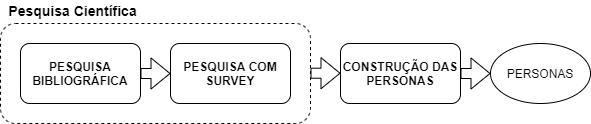
\includegraphics[keepaspectratio=true,scale=0.65]{figuras/metodologia/fluxo geral.png}
	\caption{Processo Metodológico do Trabalho - Autoral}
	\label{Fig:geral_flow.png}
\end{figure}

As atividades apresentadas na Figura \ref{Fig:geral_flow.png} seguem descritas nas seções a seguir. A Seção \ref{sec:pesq_cient} apresenta a metodologia de pesquisa bibliográfica e da pesquisa com \textit{survey} e a Seção \ref{sec:const_person} descreve o processo de construção das personas.


\section{Pesquisa Científica} 
\label{sec:pesq_cient}

Segundo \citeonline[p. 34-42]{Gerhardt2009}, a pequisa bibliográfica deste trabalho tem uma abordagem qualitativa, de natureza aplicada, com objetivo descritivo em relação aos conceitos sobre as personas, o método de criá-las e sobre as características de jogos para aprendizagem.

Esta pesquisa foi realizada de forma não sistemática, na qual foram selecionadas bases teórica \cite{barbosa_silva, BarbosaEtAl2021, cooper07} recomendadas pelos orientadores deste trabalho, a literatura utilizada no projeto de pesquisa Recursos Digitais Didáticos para Interação Humano-Computador\footnote{\url{https://github.com/RecursosDigitaisdeEnsinoAprendizagemIHC}} (RDDIHC), artigos científicos publicados \cite{deSales_SousaeSilva_2020, silva_sales_mendes2021}, resultados do projeto RDDIHC, referências encontradas a partir da leitura destes e entre outros. A interpretação e análise crítica das informações apresentadas na literatura adotada foram feitas pelo próprio autor deste trabalho \cite{ROTHER2007}. 
% O Capítulo \ref{chap:ref} apresenta o resultado dessa pesquisa bibliográfica. 

Alguns trabalhos estudados \cite{Petri_Wangenheim_2019, deSales_SousaeSilva_2020} na pesquisa bibliográfica serviram de base para a pesquisa com survey. Este segundo método de pesquisa científica utilizado no trabalho teve o objetivo de definir o público-alvo do jogo e identificar os requisitos que atendam aos objetivos deles. Segundo \citeonline{Gerhardt2009}, a abordagem desta pesquisa é quali-quantitativo, de natureza aplicada, com objetivo descritivo utilizando-se de um questionário auto-aplicável para a realização da pesquisa com \textit{survey}. 

De acordo com \citeonline{Kasunic_2005} um \textit{survey} envolve a coleta e análise de dados na qual os entrevistados respondem a um instrumento de pesquisa previamente planejado. Um \textit{survey} consiste na execução de sete atividades, como apresentado na Figura \ref{Fig:survey_flow.png}.

\begin{figure}[htbp]
	\centering
	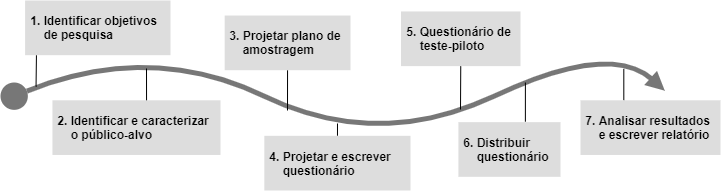
\includegraphics[keepaspectratio=true,scale=0.6]{figuras/metodologia/flow_survey.png}
	\caption{Processo de Pesquisa com Survey - Traduzido de \citeonline{Kasunic_2005}}
	\label{Fig:survey_flow.png}
\end{figure}

O processo se inicia com a identificação do objetivo de pesquisa como é apresentado na primeira etapa da Figura \ref{Fig:survey_flow.png}. O objetivo foi definido como ``caracterizar os usuários de jogos para aprendizagem'' e ``identificar a relevância dos aspectos de qualidade em jogos sérios para aprendizagem''. 

Seguindo o fluxo na Figura \ref{Fig:survey_flow.png}, na segunda etapa, identificação e caracterização do público-alvo, foi adotado nesta pesquisa a população de alunos de graduação e pós-graduação de cursos da área de Ciência da Computação. 

A terceira etapa da Figura \ref{Fig:survey_flow.png} aborda a realização do plano de amostragem, que foi definido no presente trabalho para ser realizado em instituições de ensino de graduação e pós-graduação. A coleta dos dados foi planejada para ser executada via questionário virtual, no período entre os dias 06/10/2020 e 27/10/2020. 

O questionário elaborado na quarta etapa (Figura \ref{Fig:survey_flow.png}), teve por base o modelo de personas apresentado em \citeauthor{usability2020} e por \citeonline{BarbosaEtAl2021} além das características de jogos sérios em IHC identificados por \citeonline{deSales_SousaeSilva_2020} e das metas de usabilidade e experiências do jogador descritas por \citeonline{Petri_Wangenheim_2019}. 

O questionário passou por rodadas de teste, correções e melhorias, como prescreve a quinta etapa (Figura \ref{Fig:survey_flow.png}), além de detectar quaisquer outros erros e contabilizar o tempo médio para se realizar o questionário. O teste também verificou se as questões estavam fáceis de serem entendidas e se o \textit{layout} e fluxo estavam adequados.

Na sequência, na sexta etapa (Figura \ref{Fig:survey_flow.png}), o questionário (Apêndice \ref{ap:questionario}) foi distribuído via mensagem eletrônica e redes sociais para a comunidade discente da Universidade Católica de Salvador (UCSAL), Universidade de Brasília (UnB), Universidade Federal de Uberlândia (UFU), Universidade Federal do Amazonas (UFAM),  Universidade Federal do Mato Grosso (UFMT), Universidade Federal do Mato Grosso do Sul (UFMS) e Universidade Tecnológica Federal do Paraná (UTFPR).

Na última etapa, conforme mostra a Figura \ref{Fig:survey_flow.png}, os dados coletados foram armazenados em uma planilha eletrônica e posteriormente analisados. O procedimento, o questionário, os dados e a análise completa e com mais detalhes, encontra-se no pacote de pesquisa em: \url{https://github.com/RecursosDigitaisdeEnsinoAprendizagemIHC/research-pack-hci-games}.

A partir dos dados analisados no \textit{survey} e do conhecimento adquirido na pesquisa bibliográfica, foram construídas as personas. De acordo com o processo descrito em \citeauthor{usability2020} a coleta e analise de dados sobre o público-alvo é a atividade que deve preceder a construção das personas. A seção seguinte descreve o processo de construção das personas utilizado neste trabalho.

\section{Construção das Personas}
\label{sec:const_person}

O processo de construção das personas descrito por \citeonline{cooper07} apresentam sete atividades para definir um elenco de personas. Neste trabalho estas atividades foram executadas em três etapas. A Figura \ref{Fig:construct_persona.png} demonstra uma visão geral destas etapas.

\begin{figure}[htbp]
	\centering
	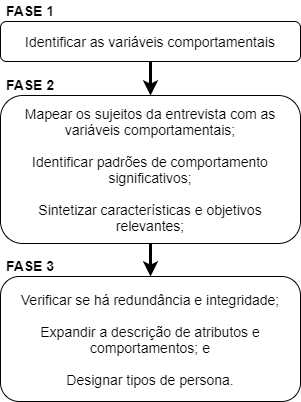
\includegraphics[keepaspectratio=true,scale=0.6]{figuras/metodologia/construct_persona.png}
	\caption{Processo de Construção das personas}
	\label{Fig:construct_persona.png}
\end{figure}


As respostas de cada indivíduo encontrava-se registrada na planilha eletrônica (PE0). Este conjunto de dados inicial foi o ponto de partida para a modelagem das personas.

Na primeira etapa foram identificadas as variáveis comportamentais. Estas foram definidas a partir das perguntas do questionário. De acordo com as respostas dadas pelos respondentes foi-se agrupando os registros de respostas dos indivíduos que tinham características comportamentais semelhantes. São estas as variáveis comportamentais, identificadas na Tabela \ref{tab:Table_variaveis-comp}.

\begin{table}[htbp]
\centering
\caption{Variáveis Comportamentais}
\label{tab:Table_variaveis-comp}
\begin{tabular}{|p{4.7cm}|p{10cm}|}
\hline
\textbf{Questão} & \textbf{Variáveis}                             \\ \hline
O01   &  Relação com a Disciplina de IHC                          \\ \hline
H01   &  Experiência com design de interfaces                      \\ \hline
RL01   &  Ação para sanar dúvidas de algum conteúdo               \\ \hline
O02  &  Uso de jogos para aprender                \\ \hline
O02.1.1, O02.2.1, O02.3.1   &  Motivos para usar jogos para aprendizagem\\ \hline
O02.1.2, O02.2.2   &  Frequência no uso de jogos para aprendizagem\\ \hline
O02.1.4  & Motivos para deixar de usar jogos para aprendizagem       \\ \hline
O02.3.2  &  Motivos de nunca ter usado jogos para aprendizagem    \\ \hline
O02.4.1  & Motivos de não ter interesse em jogos para aprendizagem       \\ \hline
RE01  & Relevância dos fatores de usabilidade do jogo          \\ \hline
E01   & Importância dos fatores de experiência do jogo        \\ \hline
\end{tabular}
\legend{Fonte: Autor}
\end{table}

A Tabela \ref{tab:Table_variaveis-comp} relaciona o identificador de uma questão do formulário, segunda coluna, com as respectivas variáveis comportamentais, na primeira coluna da mesma tabela. As perguntas utilizadas para levantar essas variáveis encontram-se na Tabela \ref{tab:quest-survey}.  
% \begin{itemize}
%     \item I01 [Idade], I02 [sexo] e I03 (Figura \ref{Fig:survey_pt2.png}): complementa a caracterização da persona, dando aspectos mais reais a ela;
%     \item I04 (Figura \ref{Fig:survey_pt2.png}): pode evidenciar um certo grau de conhecimento mais técnico entre os usuários que cursam graduação na área de Ciência da Computação e os de outros cursos;
%     \item O01 (Figura \ref{Fig:survey_pt3.png}): pode evidenciar um certo grau de conhecimento e experiência do usuário em relação a área de Interação Humano-Computador;
%     \item H01 (Figura \ref{Fig:survey_pt3.png}): pode evidenciar um certo grau de conhecimento e experiência mais prática em IHC;
%     \item H02 (Figura \ref{Fig:survey_pt4.png}): pode evidenciar um certo grau de conhecimento e experiência mais prática em IHC;
%     \item RL01 (Figura \ref{Fig:survey_pt5.png}): ajuda a apontar os relacionamentos mais relevantes do usuário no contexto de ensino e aprendizagem, que serve para identificar uma oportunidade de intervenção em que um jogo educacional pode auxiliar nessas relações;
%     \item O02 (Figura \ref{Fig:survey_pt5.png}): quesito base que evidencia o nível de afinidade do usuário com jogos para aprendizagem;
%     \item O02.1.1 (Figura \ref{Fig:survey_pt6.png}), O02.2.1 (Figura  \ref{Fig:survey_pt7.png}) e O02.3.1 (Figura \ref{Fig:survey_pt8.png}): quesito que evidencia o objetivo do usuário ao usar um jogo educacional;
%     \item O02.1.2 (Figura \ref{Fig:survey_pt6.png}) e O02.2.2 (Figura \ref{Fig:survey_pt7.png}): auxilia na percepção da frequência em que os usuários costumam usar jogos para aprendizagem;
%     \item O02.1.4 (Figura \ref{Fig:survey_pt6.png}): auxilia na identificação de usuários específicos que têm uma afinidade relevante para com os jogos para aprendizagem; 
%     \item O02.3.2 (Figura \ref{Fig:survey_pt8.png}) e O02.4.1(Figura \ref{Fig:survey_pt9.png}): auxilia na complementação das características das anti-personas
%     \item RE01 (Figura \ref{Fig:survey_pt10.png}) e E01 (Figura \ref{Fig:survey_pt11.png}): serve para identificar a preferencia dos usuários em relação às características e experiências dos jogos para aprendizagem;
% \end{itemize}

Após a identificação das variáveis comportamentais seguiu-se para a Etapa 2 como é apresentado na Figura \ref{Fig:construct_persona.png}. Os passos foram o mapeamento dos respondentes em relação a essas variáveis, a identificação de padrões de comportamento significativos e a sintetização de características e objetivos relevantes.

Fez-se uso da planilha eletrônica (PE0) e suas ferramentas para a auxiliar o processo de filtragem e síntese dos dados. Primeiramente foram divididos em dois, os dados dos respondentes, a partir da variável I04. Assim foi definida a estrutura base da anti-persona (PE2), aqueles que não são da área de Ciência da Computação, e também a estrutura base das demais personas (PE1). Na Figura \ref{Fig:persona_tree.png} é apresentada o processo de refino dos dados para construção das personas.

\begin{figure}[htbp]
	\centering
	\caption{Fluxo do processo de construção das personas}
	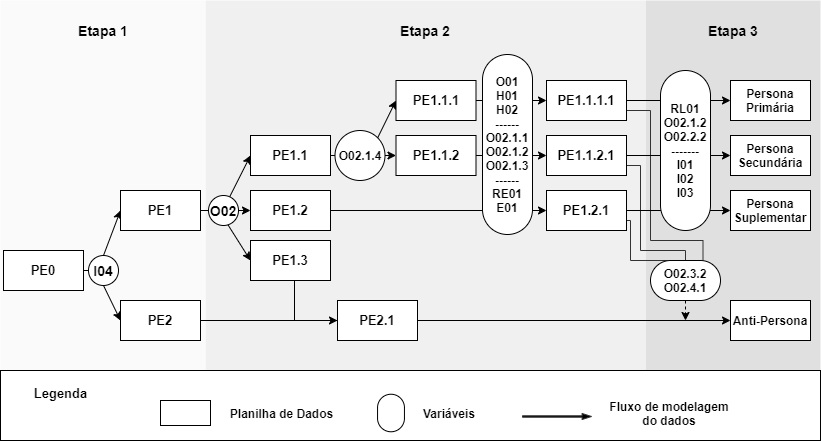
\includegraphics[keepaspectratio=true,scale=0.55]{figuras/metodologia/persona_tree.png}
	\label{Fig:persona_tree.png}
\end{figure}

\newpage

A partir da variável O02 foi possível agrupar os dados em três perfis comportamentais, a partir dos dados em PE1. Foram estes, o perfil daqueles que ainda usavam jogos e os que já usaram, mas não jogavam mais (PE1.1); o perfil  daqueles que nunca jogaram, mas tinham um interesse (PE1.2); e o perfil daqueles que não tinham interesse de jogar (PE1.3). Este último (PE1.3) foi englobado ao PE2, formando o PE2.1.

Dentro de PE1.1 existiam aqueles que já haviam jogado, mas por algum motivo tinham parado de usar jogos para aprendizagem. Destes foram relevantes para o objetivo do trabalho apenas aqueles que pararam de jogar por terem alcançado seu objetivo por meio do jogo para aprendizagem. Foi obtido então PE1.1.1, com  os dados daqueles que usavam jogos para aprendizagem e PE1.1.2, aqueles que haviam jogado, mas pararam por haverem alcançado seu objetivo de estudo, que no caso foram identificados pela variável O02.1.4.

O próximo passo foi identificar, a partir das variáveis H01, H02 e O01, quais os perfis comportamentais seriam mais frequentes para compor personas significativas. Nesta análise, os perfis comportamentais identificados expressavam que os respondentes tinha um conhecimento raso sobre IHC ou nenhum conhecimento, sendo que estes ou estavam fazendo o curso de IHC ou ainda não haviam feito.

Agrupados esses conjuntos de características foi possível definir os objetivos das personas (O02.1.1, O02.2.1 e O02.3.1). A busca por um jogo que auxilie no aprendizado de um conteúdo novo, um jogo que ajude na revisão de um conteúdo visto e um que forneça a possibilidade de avaliar o conhecimento do jogador, formando então os perfis PE1.2.1, PE1.1.1.1 e PE1.1.2.1. Com os objetivos definidos, foi então identificada a experiência e elementos do jogos (RE01 e E01) mais relevantes buscados por cada um dos três perfis. 

Com essa estrutura base das personas, foi realizada a terceira e última etapa (Figura \ref{Fig:construct_persona.png}), que visa lapidar as personas. Foi verificada a integridade das personas e se existiam redundâncias entre elas. Uma descrição mais detalhada de atributos e comportamentos foram inseridos, tirando como base as seguintes variáveis RL01, O02.1.2, O02.2.2, I01, I02 e I03). Estas serviram para dar mais realismo às personas, além de terem recebido uma foto de perfil cada. 

Por fim foram designados os tipos de personas, primária, secundária e suplementar. No caso das características da anti-persona, as variáveis O02.3.2 e O02.4.1 auxiliaram a complementá-la, além dos atributos que foram considerados como irrelevantes para as outras personas.

O processo de construção com mais detalhes encontra-se em: 
\url{https://github.com/RecursosDigitaisdeEnsinoAprendizagemIHC/research-pack-hci-games}, tal como os resultados. No Capítulo \ref{chap:result} estão apresentados estes resultados e sua análise.

%%%% E aquela parte onde vc calculou o peso de cada um dos requisitos de qualidade???